\section{In Search for Linear Relations in Sentence Embedding Spaces}
\label{section:semantic_space}

In this section,\footnote{This section is based on the article \citep{barancikova-bojar-linear}, a joint work with Ondřej Bojar. The methodology and experimental framework is adapted from the original study, however, all experiments with the exception of \Cref{sect:visualization:elmo} are recomputed using updated scripts and an updated set of sentence embedding model. As a result, reported numbers may differ from those published in the original article.} we investigate whether sentence embedding spaces exhibit consistent linear structure, analogous to the well-known properties of word embeddings. A notable observation by \cite{word2vec} demonstrated that meaningful relationships between words have immediate geometric counterparts in the continuous vector space. \cite{word2vec} defined a series of tests to measure how well word embeddings capture semantic and syntactic information. These tests include, for example, declination of adjectives (``easy"$\rightarrow$``easier"$\rightarrow$``easiest"), changing the tense of a verb (``walking"$\rightarrow$``walk") or matching a capital to a corresponding country (``Athens"$\rightarrow$``Greece") or currency (``Angola"$\rightarrow$``kwanza").

\begin{figure}[t!]
  \centering
  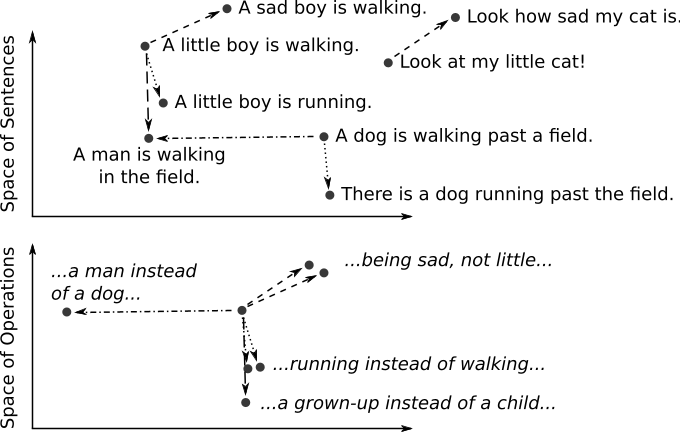
\includegraphics{spaces.png}
\caption{An illustration reprinted from \cite{barancikova-bojar-linear}. The upper plot represents a continuous multi-dimensional vector space where individual sentences are represented as points (the ``space of sentences''). Pairs of related sentences are connected by arrows, with different dashing styles indicating various relationship types.\\
The lower plot illustrates the corresponding ``space of operations.'' Here, a vector difference is shown, with all arrows moved to start at a common origin. \\
The underlying hypothesis is that consistent semantic changes (e.g., all vector transformations extracted from sentence pairs differing in the speed of travel ``running instead of walking'') should be represented close to each other in the space of operations, i.e., form a more or less compact \emph{cluster}.}
\label{space-of-sentences}
\end{figure}

Our objective is to determine whether \emph{whole sentence} embeddings exhibit the same linear behavior, looking for an analogous behavior to that observed with word embeddings. This idea is illustrated in \cref{space-of-sentences}. Specifically, we examine whether semantic shifts between sentences can be modeled as transformation vectors. Understanding whether sentence embeddings exhibit consistent linear structure is particularly important for embedding-based evaluation metrics, which implicitly rely on geometric properties such as vector similarity and compositionality.

Following \cite{word2vec}, we deliberately do \emph{not include} this aspect in the training objective of the sentence representations, but instead search for properties that are learned in an unsupervised way, as a side-effect of the original training objective, data and setup. This approach has the potential to \emph{explain} good or bad performance of the representation types examined in various tasks.

We acquire pairs of sentences that differ by small alterations (such as a change of noun, the addition of an adjective, or punctuation) from natural language inference datasets. Throughout this section, we refer to the original sentence as the premise ($P$) and the modified sentence as the hypothesis ($H$), following the NLI terminology. We hypothesize that if $P$ and $H$ represent two sentences differing only by a single linguistic edit (e.g., \pattern{X man Y}{X woman Y}), the operation between their representation in vector space, e.g., $ V_{trans} = V_{H} - V_{P}$  should isolate that specific edit in a consistent direction across the vector space.

In particular, we proceed in the following steps:
\begin{enumerate}
    \item \textbf{collect sentence pairs:} Each pair consists of a premise and a hypothesis that differ by a specific small alteration (the modification pattern). The process of collecting such pairs of sentences is described in detail in \Cref{examined-sentences}.
    \item \textbf{compute sentence embeddings:} Each sentence is embedded in a vector space using various sentence embedding models. We use a representative subset of sentence embeddings that are introduced in \cref{examined-embeddings},   
    \item \textbf{compute vector operations:} Apply arithmetic operations to the embeddings of this pair of sentences to capture the transformation between them, i.e., their \textit{transformation vectors}. The operations used are presented in \Cref{operations}.
    \item \textbf{cluster transformation vector and evaluate clustering:} For evaluation, we first use the k-Means algorithm for clustering to group transformation vectors based on their position in the space of operations. In order to see how well the clusters correspond to the actual modification patterns, we evaluate them using cluster evaluation metrics. Clustering metrics and evaluation are described in more detail in \Cref{clustering_metrics} and \Cref{sect:lin-spaces:analysis}, respectively.
\end{enumerate}

\begin{mdframed}[
    linecolor=gray,
    linewidth=2pt,
    roundcorner=5,
    backgroundcolor=gray!5
]
\noindent
In this chapter, we investigate whether sentence embedding spaces exhibit linear semantic structure analogous to that observed in word embeddings, focusing on the following research questions:

\begin{itemize}
    \item Can semantic and syntactic transformations between sentences be captured through simple arithmetic operations in continuous vector spaces?
    \item To what extent do model architecture and scale influence the linearity of the sentence embedding space?
    \item Is the linearity of a model the result of a learned semantic understanding or an inherent inductive bias of its architecture
    \item Which linguistic phenomena are most (and least) consistently represented as linear transformations in sentence embeddings?
\end{itemize}
\end{mdframed}

%We present introductory investigation into a continuity of a multidimensional 
%vector space of sentences. In this research, we would like to look into 
%how even a small change (such a negation, change of tense, generalization) 
%in a sentence affects its representation and whether these changes are coherent 
%across a vector space or how to create a vector space with such a property.

%However, obtaining such a data in good quality is time and money consuming. 
%Therefore, we started with a smaller scale experiment using existing data for 
%natural language inference (NLI). We selected slightly different sentences 
%using simple pattern method (see \cref{pattern_method}). The patterns are 
%actually not that common in data, but they represent a good example of 
%real-word sentences differing just by a small alternations.


\subsection{Sentence Patterns}
\label{examined-sentences}

\begin{figure}[hb!]
\begin{tabular}{cl}
\toprule
\textbf{Step} & \textbf{Premise and hypothesis} \\ 
\midrule
0. & $P$: a man with a tattoo behind his \textbf{ear is playing a guitar.} \\
   & $H$: a woman with a tattoo behind her \textbf{ear is playing a guitar.} \\ 
   
1. & $P_1$: a man \textbf{with a tattoo behind} his $X$ \\
   & $H_1$: a woman \textbf{with a tattoo behind} her $X$ \\ \
   
2. & $P_2$: a man $Y$ his $X$ \\
   & $H_2$: a woman $Y$ her $X$ \\ 
   
3. & $P_3$: a man $X$ his $Y$ \\
   & $H_3$: a woman $X$ her $Y$ \\ 
\bottomrule
\end{tabular}
\caption{Example of our pattern extraction method. In step~0, the longest common substring of tokens (\textit{ear is playing a guitar .}) between the original premise $P$ and original hypothesis $H$ is identified and replaced with the variable $X$ in step~1. In step~2, \textit{with a tattoo behind} is identified as the longest common substring and substituted with the variable $Y$. As the variables are not listed alphabetically in the premise, they are switched in step~3, which also yields the final pattern \pattern{a man X his Y}{a woman X her Y}.}
\label{tab:howisitdone}
\end{figure}

Because manual creation of sentence variations is costly, we reuse existing English data from the Stanford Natural Language Inference Corpus (SNLI) \citep{snli} and Multi-Genre Natural Language Inference (MultiNLI)  \citep{MultiNLI}. Both collections consist of pairs of sentences, a premise and a hypothesis, and their relationship (entailment, contradiction, or neutral). The two datasets together contain almost one million unique sentence pairs. All sentences were lowercased and tokenized using the NLTK library \citep{nltk}.

From the available data, we select only a subset where the difference between sentences in a pair can be described with a simple pattern. We adopt the following approach: given a premise  $P$ and a corresponding hypothesis  $H$, we identify the longest common substring consisting of whole words and replace it with a variable $X$. This step is repeated once more, allowing our sentence patterns to contain up to two variables $X$ and $Y$. In the last step, we make sure that the pattern is in canonical form by renaming the variables to ensure that the variable $X$ always precedes $Y$ within the premise  $P$. The process is illustrated in \cref{tab:howisitdone}.

The ten most common patterns for each NLI relation are shown in \cref{patterns}. Many of the obtained patterns clearly match the sentence pair label. For example, the entailment patterns are mainly generalizations and change of the word order, while the contradiction patterns show typical oppositions like man--woman, dog--cat. Neutral pairs often represent various refinements of the content, likely due to the original SNLI instruction that a hypothesis ``might be true'' given the premise in a neutral relation.

\begin{figure}[H]
\centering

% Entailments Table
\begin{tabular}{l r}
\multicolumn{2}{c}{\textbf{Entailment}} \\ 
\toprule
\textbf{Pattern} & \textbf{Count} \\ 
\midrule
\pattern{X}{X}                 & 693 \\
\pattern{X man Y}{X person Y}     & 224 \\
\pattern{X .}{X}               & 207 \\
\pattern{X woman Y}{X person Y}   & 118 \\
\pattern{X boy Y}{X person Y}     & 65  \\
\pattern{X Y}{Y , X .}         & 61  \\
\pattern{X men Y}{X people Y}     & 56  \\
\pattern{two X}{X}             & 56  \\
\pattern{X girl Y}{X person Y}    & 55  \\
\pattern{X , Y}{Y X .}         & 53  \\ 
\bottomrule
\end{tabular}

\vspace{0.85cm}

% Contradictions Table
\begin{tabular}{l r}
\multicolumn{2}{c}{\textbf{Contradiction}} \\ 
\toprule
\textbf{Pattern} & \textbf{Count} \\ 
\midrule
\pattern{X man Y}{X woman Y}   & 413 \\
\pattern{X woman Y}{X man Y}   & 196 \\
\pattern{X men}{X women Y}     & 111 \\
\pattern{X boy Y}{X girl Y}    & 109 \\
\pattern{X dog Y}{X cat Y}     & 98  \\
\pattern{X girl Y}{X boy Y}    & 97  \\
\pattern{X women Y}{X men Y}   & 64  \\
\pattern{X Y,}{X not Y}        & 56  \\
\pattern{two X,}{three X}      & 46  \\
\pattern{X child Y}{X man Y}   & 44  \\ 
\bottomrule
\end{tabular}

\vspace{0.85cm}

% Neutrals Table
\begin{tabular}{l r}
\multicolumn{2}{c}{\textbf{Neutral}} \\ 
\toprule
\textbf{Pattern} & \textbf{Count} \\ 
\midrule
\pattern{X Y}{X sad Y}         & 701 \\
\pattern{X Y}{X big Y}         & 119 \\
\pattern{X Y}{X fat Y}         & 69  \\
\pattern{X young Y}{X sad Y}   & 68  \\
\pattern{X people Y}{X men Y}  & 60  \\
\pattern{X}{sad X}             & 51  \\
\pattern{X}{X}                 & 41  \\
\pattern{X person Y}{X man Y}  & 34  \\
\pattern{X Y}{X red Y}         & 30  \\
\pattern{X Y}{X busy Y}        & 28  \\ 
\bottomrule
\end{tabular}

\caption{Top 10 patterns extracted from sentence pairs labeled as entailment, contradiction, and neutral, respectively.}
\label{patterns}
\end{figure}

\pagebreak
We keep only patterns within at least 20 different sentence pairs in the datasets in order to have large and variable sets of sentence pairs in subsequent experiments. We also excluded the most common pattern---identity---as it does not alter the sentence. Surprisingly, identity is not just among entailment pairs (693 cases), but also in neutral (41 cases) and contradictory (22) pairs, showing label noise or human error in the original datasets.

In total, we collected 4,200 unique sentence pairs across 60 patterns. Approximately 10\% of this data originates from MultiNLI, with the majority derived from SNLI.


\subsection{Sentence Embeddings}
\label{lin:examined-embeddings}
In this chapter, we evaluate the linear properties in the diverse set of sentence embedding models introduced in detail in \Cref{examined-embeddings}. These include legacy architectures (\infersent, \elmo, \useemb), modern Transformer-based models (\bertlarge, \sbert, \modernbert, \ensimcse), multilingual variants (\labse , \bgemthree, \laser), and recent instruction-tuned encoders (\elarge, \esmall), LLM-based decoder (\qwen ), proprietary models (\tetrismall, \tetrilarge, \geminiemb). As control models, we use \random and \enrandombert. For complete specifications, dimensions, training objectives, see \Cref{examined-embeddings} and \Cref{tab:model_comparison_detailed}.

Although \Cref{tab:model_comparison_detailed} lists 26 embedding models, only a subset of 18 models is used in the experiments presented in this section. This selection is motivated by the experimental setup: the analysis of linear properties of embedding spaces is conducted exclusively on English data, and Czech-specific models are therefore excluded. In addition, we exclude \xlmr 
due to its strong anisotropy and poor performance in semantic similarity (as shown further in \cref{extrinsic}), and \mepet as it was introduced only in later stages of this work.


\subsection{Choosing Vector Operations}
\label{operations}
\cite{word2vec} used a simple vector difference as the operation that relates two word embeddings. For sentences embeddings, we experiment with four simple operations: addition, subtraction, multiplication and division, all applied element-wise to a pair of embedding vectors. More operations could be also considered as long as they are reversible, so that we can isolate the vector change for a particular sentence alternation and apply it to the embedding of any other sentence. Hopefully, we would then land in the area where the correspondingly altered sentence is embedded.

The underlying idea of our analysis was already sketched in \cref{space-of-sentences}. From every sentence pair in our dataset, we extract the modification pattern, i.e., the specific change made from one sentence to the other (e.g., changing a noun, adding an adjective, or negation). The arithmetic operation needed to move from  the embedding of the first sentence to the embedding of the second sentence (in the continuous space of sentence embeddings) can be represented as a point in what we call the \emph{space of operations}. 


\subsection{Evaluation Metrics}
\label{clustering_metrics}

Considering all sentence pairs that share the same modification pattern, we obtain many points in the space of operations. If the sentence embedding space reflects the particular modification pattern in an accessible way, all the corresponding points in the space of operations will be close together, forming a cluster. To evaluate the clustering of sentence transformation vectors, we test patterns with a metric suite designed to capture the information-theoretic, pairwise, and geometric properties of the resulting clusters:

\begin{itemize}
    \item \textbf{Adjusted Mutual Information (AMI)} \citep{JMLR:v11:vinh10a} measures the information shared in cluster assignments; specifically, it calculates how much uncertainty about ground-truth labels is reduced by knowing the cluster assignments. It typically ranges between 0 and 1, where 1 indicates that the clusters perfectly match the ground truth. Note that AMI can take slightly negative values due to chance correction; values close to zero (including small negative values) indicate performance equivalent to random clustering.
    The correction for chance ensures that random label assignments do not artificially inflate the success score, a common problem in experiments involving a large number of clusters \citep{JMLR:v11:vinh10a}, such as the 60 distinct sentence patterns used in this experiment. 

    \item \textbf{Adjusted Rand Index (ARI)} \citep{Hubert1985} measures pairwise accuracy --  it evaluates every possible pair of data points and determines whether their co-occurrence in a cluster matches their co-occurrence in the ground truth. The score ranges from -1 to +1, with 1 being the perfect match score and values around 0 meaning random label assignment. Negative numbers indicate worse agreement than a random result due to systematic disagreement. By reporting both AMI and ARI, we can distinguish between models that correctly identify general "neighborhoods" of transformations and those that achieve high-fidelity membership accuracy across all 60 patterns.

    \item \textbf{Silhouette Coefficient} \citep{Rousseeuw:1987} is employed to analyze the internal geometric separation of the vectors within the embedding space. Using a cosine distance metric, the Silhouette score measures the ratio of intra-cluster cohesion to inter-cluster separation, providing a label-independent validation of the cluster structure. A high Silhouette score confirms that the linguistic patterns are mapped into isolated "islands" rather than a continuous, overlapping distribution. Given that sentence embeddings typically reside on a high-dimensional hypersphere, the use of a cosine-based Silhouette score is more semantically appropriate than Euclidean distance for assessing the density and separation of the transformation vectors.

    \item \textbf{Intra-Cluster Cosine Similarity} is used to validate the consistency of the vector arithmetic. This metric calculates the mean directional alignment of all transformation vectors (e.g., \pattern{X child Y}{X man Y}) within a specific pattern. \cite{mikolov-etal-2013-linguistic} shows that a high consistency score demonstrates that a linguistic transformation maintains a parallel trajectory across diverse lexical contexts All transformation vectors are L2-normalized prior to cosine similarity computation. This normalization is particularly important as most embedding models are optimized for cosine similarity rather than Euclidean distance.
       
    % \item \textbf{V-measure} \cite{vmeasure} is the harmonic mean of \textit{homogeneity} (each 
    % cluster should contain only members of one class) and \textit{completeness} (all members 
    % of one class should be assigned to the same cluster). The score ranges from 0 (the worst
    % case) to 1 (perfect score). 
 \end{itemize}   


%We experiment with two more metrics -- V-Measure and the Davies-Bouldin Index; however, they are excluded from the final reporting due to redundancy. Our preliminary analysis reveals that these metrics are nearly perfectly correlated with AMI and Silhouette, respectively.

\subsection{Comparative Analysis of Vector Operations}
\label{sect:lin-spaces:analysis}

We use these metrics to evaluate how well a clustering algorithm can recover known sentence modification patterns in different sentence embedding spaces. Although clustering is performed in an unsupervised manner, fixing the number of clusters to the number of known patterns introduces a mild form of supervision, allowing us to directly evaluate alignment with ground-truth transformations.

To ensure clarity, let's outline the design of the experiment once again. First, sentence embeddings were computed using the selected models (Sect. 4.3.2) and  L2-normalized; normalization ensures that transformation vectors (calculated in the upcoming step) capture directional semantic change rather than magnitude differences. 
Second, for each pair of sentences, transformation vectors were computed using addition, subtraction, multiplication, and division, applied element-wise, as described in \Cref{operations}.
Third, transformation vectors were clustered using k-Means with the number of clusters fixed to the number of ground-truth patterns (i.e., 60), using the scikit-learn implementation \citep{scikit-learn}. 

Finally, we compare the resulting cluster assignments to the gold truth labels using AMI, ARI, and the Silhouette score. To reduce variance due to random cluster initialization, we report the best clustering obtained over 100 random restarts. High agreement between predicted clusters and ground-truth patterns indicates that the corresponding linguistic transformations are encoded in a consistent and separable manner within the sentence embedding space.

\begin{table}[tb]
    \centering
        \begin{tabular}{rrrrrr}
        \toprule
        operation & AMI & ARI & Silhouette & Cosine mean $\pm$ std \\
        \midrule
        $-$      & 0.82 & 0.48 & 0.29 & 0.63  $\pm$ 0.25 \\
        $+$      & 0.19 & 0.04 & -0.06 & 0.51 $\pm$ 0.06 \\
        $\times$ & 0.15 & 0.03 & -0.08 & 0.65 $\pm$ 0.03 \\
        $/$ &    -0.00 & -0.00 & -0.03 & 0.03  $\pm$ 0.04 \\       
        \bottomrule
        \end{tabular}
    \caption{Averaged performance of cluster evaluation metrics over all evaluated models.}
    \label{tab:mean_operations}
\end{table}

To identify the optimal mathematical representation of linguistic transformations, we evaluated four primary vector operations: addition ($+$), subtraction (-), multiplication ($\times$) and division ($/$). \Cref{tab:mean_operations} presents the performance of these operations, averaged across all sentence embedding models (excluding random BERT and random).

The experimental results show that the best cluster distribution is achieved by far using the most intuitive operation, vector subtraction. Subtraction achieved AMI of 0.82 and ARI of 0.48, significantly higher than the scores produced by other operations. Notably, subtraction is the only operation that resulted in a positive Silhouette score (0.29), indicating that it produces actual cluster separation rather than a disordered distribution of points. However, the relatively high standard deviation suggests that the consistency of transformation directions varies substantially across patterns, indicating that not all linguistic phenomena are equally well captured by linear operations.

From a theoretical perspective, the success of subtraction supports the \textit{transformation vector} hypothesis \citep{mikolov-etal-2013-linguistic, VylomovaRCB15}. If sentence embeddings are structured linearly, the difference vector $V_{trans} = V_{H} - V_{P}$ approximates the removal of shared semantic content and isolates the specific linguistic shift. The high AMI score confirms that this resulting vector retains highly specific information about the transformation, while the positive Silhouette score provides strong evidence that these shifts occupy distinct regions in the vector space.
 
In contrast, addition and multiplication fail to produce a meaningful clustering structure. Although addition ($+$) yields a relatively high intra-cluster cosine similarity (0.51), its negative Silhouette score (-0.06) and low ARI (0.04) reveal that it does not create distinct boundaries. The addition combines the semantics of both sentences into a "centroid" representing the sum of all parts; it doubles the context rather than isolating the change. Consequently, the resulting vectors for different patterns overlap in a single semantic mass, making them indistinguishable from clustering algorithms.

Multiplication ($\times$) and division ($/$) are even less effective. Multiplication is sensitive to the magnitude of specific dimensions and does not align with the directional, cosine-based logic on which modern transformer embeddings are optimized. Interestingly, multiplication yields relatively high intra-cluster cosine similarity despite poor clustering performance. This suggests that multiplication produces vectors with similar magnitudes and directions, but without meaningful separation between different transformation types. In other words, it creates globally consistent but non-discriminative representations. Division fails to preserve directional information and produces results indistinguishable from random clustering, as evidenced by an AMI of -0.00, which is functionally equivalent to random chance.

These results suggest that further analysis of addition, multiplication, or division is unlikely to yield meaningful insights.
These operations fail to uncover the latent structural regularities of the pattern in embedding spaces, their transformation vectors behaving largely as random noise. However, results for subtraction suggest that the transformation between related sentences is encoded as a consistent directional shift. Therefore, in the rest of the chapter, we focus entirely on subtractions. In the next section, we compare subtraction results in more detail from different architectures—from legacy LSTMs to modern Transformers. 

\subsection{Detailed Results: Selected Embedding Models}

Across all trained sentence embedding models, vector subtraction produces compact and well-separated clusters that align closely with the corresponding sentence transformation patterns. As shown in \Cref{tab:linear_subtraction}, semantically trained models achieve high AMI and ARI, indicating strong agreement between clustered transformation vectors and ground-truth labels. 

This behavior is robust in various model families, including BiLSTM-based encoders (\infersent), encoder-only Transformers (\sbert, \bgemthree), multilingual models (\labse) and proprietary embedding services (\hbox{\tetrismall{}}). The lack of a clear performance gap between model families suggests that the ability to encode sentence-level transformations as linear directions is a robust and widely shared property of modern sentence embedding spaces.

\begin{table}[]
    \centering
        \begin{tabular}{lccccc}
        \toprule
        name & AMI & ARI & Silhouette & Cos. mean $\pm$ std & RandCos \\
        \midrule
        \infersent & \textbf{0.87} & 0.54 & 0.35 & 0.65  $\pm$  0.22 & 0.54 \\
        \tetrilarge & 0.86 & 0.56 & 0.26 & 0.54  $\pm$  0.22 & 0.14 \\
        \tetrismall & 0.86 & 0.56 & 0.31 & 0.61  $\pm$  0.24 & 0.15 \\
        \sbert & 0.84 & 0.49 & 0.36 & 0.72  $\pm$  0.28 & 0.05 \\
        \geminiemb & 0.84 & 0.52 & 0.27 & 0.60  $\pm$  0.26 & 0.59 \\
        \labse & 0.84 & \textbf{0.59} & 0.32 & 0.76  $\pm$  0.22 & 0.48 \\
        \elarge & 0.83 & 0.52 & 0.28 & 0.65  $\pm$  0.27 & 0.72 \\
        \qwen & 0.83 & 0.44 & 0.31 & 0.64  $\pm$  0.28 & 0.26 \\
        \ensimcse & 0.83 & 0.50 & 0.27 & 0.70  $\pm$  0.24 & 0.36 \\
        \esmall & 0.83 & 0.45 & 0.38 & 0.76  $\pm$  0.26 & 0.78 \\
        \bgemthree & 0.82 & 0.41 & 0.36 & 0.72  $\pm$  0.27 & 0.62 \\
        \elmo & 0.82 & 0.48 & 0.33 & 0.61  $\pm$  0.21 & 0.52 \\
        \modernbert & 0.82 & 0.52 & 0.33  &  0.64 $\pm$ 0.27 & 0.49 \\
        \laser & 0.76 & 0.45 & 0.23 & 0.45  $\pm$  0.24 & 0.60 \\
        \bertlarge & 0.72 & 0.38 & 0.12 & 0.41  $\pm$  0.17 & 0.50 \\
        \enrandombert & 0.71 & 0.45 & \textbf{0.46} & 0.62  $\pm$  0.34 & 0.95 \\
        \useemb & 0.70 & 0.24 & 0.13 & 0.66  $\pm$ 0.28 & 0.17 \\
        \random & 0.00 & 0.00 & -0.03 & 0.00  $\pm$  0.00 & -0.00 \\
        \bottomrule
        \end{tabular}
        
    \caption{Result of different models based on the subtraction. In the RandCos column, we state Cosine similarity between two random sentence vectors from our dataset averaged over one thousand runs.}
    \label{tab:linear_subtraction}
\end{table}

Interestingly, our experiment shows that the model scale is not a reliable predictor of the linear semantic structure. Although the scaling laws of Transformer-based model accurately predict improvements in linguistic modeling and downstream task performances \citep{kaplan2020scalinglawsneurallanguage}, this does not necessarily translate into a more structured geometric space for vector arithmetic. As shown in \Cref{tab:linear_subtraction}, \sbert with 23M parameters performs comparably to substantially larger decoder-only architectures (e.g., \geminiemb). This finding suggests that semantic alignment is driven less by model size than by the training objective. In particular, contrastive supervision appears to impose a form of geometric pressure that organizes linguistic transformations into consistent directional shifts—an emergent property that does not arise naturally from large-scale next-token prediction alone.

Interestingly, among the best performing models are not just modern methods, but also \infersent, a legacy architecture, which yielded an AMI of 0.87 and a Silhouette score of 0.35.  However, we interpret this not as a sign of superior architecture, but as task-specific overfitting. \infersent was trained specifically on the SNLI dataset from which our patterns are derived. Furthermore, \cite{dasgupta2018} investigated the compositionality in sentence embedding spaces and found that \infersent relies strongly on shallow word-level heuristics rather than exhibiting genuine compositional understanding. Supporting this conclusion, \cite{mccoy-etal-2019-right, gururangan-etal-2018-annotation} found that \infersent (and early transformers to some extent) exploit superficial statistical regularities in SNLI rather than learning robust entailment. Consequently, if transformations at the word-vector level are minimal, then the difference between two sentence embeddings is strongly influenced by the embedding of the underlying transformation pattern. This observation provides a plausible explanation for why such patterns are consistently clustered together in the embedding space.  In summary, our results are not evidence that \infersent is a superior general-purpose sentence encoder, but rather strong evidence consistent with task-specific overfitting. 

The large variation in cosine similarity between randomly selected sentence vectors (RandCos) reflects fundamental differences in the global geometry of embedding spaces across models. High RandCos values indicate strong anisotropy, where sentence representations occupy a narrow region of the space and are therefore highly similar regardless of their content. Conversely, lower values suggest a more uniform distribution of vectors across the space. Importantly, this property is largely independent of clustering performance. \elarge with high anisotropy still achieve strong clustering results, indicating that meaningful transformation directions can exist even in geometrically compressed spaces. At the same time, lower anisotropy does not automatically guarantee better separability of transformation patterns. This suggests that global space geometry and the ability to encode consistent transformation directions are related but distinct properties of sentence embeddings.


In our control experiments, \random does not exhibit any meaningful structure, while \enrandombert unexpectedly generates moderately well-separated clusters and notably the highest Silhouette coefficient. However, this result does not represent genuine semantic understanding. The high cosine similarity of the random sentence embeddings (0.95) suggests very high anisotropy. However, the model still encodes small, consistent \textit{micro-shifts} in response to systematic linguistic modifications in the input sentences. These micro-shifts arise from a combination of factors: the tokenizer, trained on large corpora, introduces subtle language-derived structure by consistently mapping similar linguistic patterns to similar token sequences (or to systematic differences in those sequences); meanwhile, the Transformer architecture—even with random weights—reacts to these structured input variations through its attention and feed-forward mechanisms, amplifying small differences into detectable linear patterns. Therefore, we can consider \enrandombert to be an upper bound on the contribution of architecture and tokenizer alone. 

Compared to this architectural baseline, semantically trained models exhibit both stronger alignment with ground-truth transformation labels and more stable directional consistency. These results demonstrate that the linear structure observed in trained sentence embeddings is not an artifact of high dimensionality or model architecture, but a learned property induced by semantic training objectives.

% As detailed description of this measures is out of scope of this article, we refer readers
% to related literature (e.g. \inparcite{bonaccorso2017machine}, \inparcite{Ayad:2011}).  
% All these methods are actually designed to evaluate the optimal number of clusters. We already 
% have the ideal number of clusters -- the number of patterns, so we used the scores to compare 
% how well different arithmetic operations separated the vector spaces. 

% \begin{itemize}
%     \item \textbf{Davies-Bouldin’s index} \citep{Davies} is a function of the ratio of the sum of within-cluster distribution to between-cluster separation.  The lower the index, the better the cluster separation.
%     \item \textbf{Calinski–Harabasz score} \citep{calinski1974} is computed as a ratio between inter-clusted dispersion and intracluster dispersion. It gives a high score to well separated (high intercluster dispersion) dense agglomerates (low intracluster dispersion). The higher the score, the better designed clusters.
%     \item The \textbf{Silhouette Coefficient} \citep{Rousseeuw:1987} again measures of compactness and separation of the clusters. It awards "maximum internal cohesion and maximum cluster separation". The score ranges from -1 to $$+$$1 with positive numbers indicating compact clusters that are far from each other, while negative numbers suggest wrong cluster assignment. 
% \end{itemize}

% As detailed description of this measures is out of scope of this article, we refer readers
% to related literature (e.g. \inparcite{bonaccorso2017machine}, \inparcite{Ayad:2011}).  
% All these methods are actually designed to evaluate the optimal number of clusters. We already 
% have the ideal number of clusters -- the number of patterns, so we used the scores to compare 
% how well different arithmetic operations separated the vector spaces. The results are presented 
% in \cref{tab:davies-bouldin}. It is apparent that the best distribution is achieved using the 
% most intuitive operation -- subtraction.
% % \begin{table*}[]
% \begin{tabular}{lllllllllllll}
%                                             & \multicolumn{4}{c}{Davies-Bouldin index}       & \multicolumn{4}{c}{Calinski-Harabasz score}        & \multicolumn{4}{c}{Silhouette score}               \\ \hline
% \multicolumn{1}{|l}{embedding}              & -    & $+$    & *    & \multicolumn{1}{l|}{/}    & -      & $+$     & *     & \multicolumn{1}{l|}{/}    & -     & $+$     & *     & \multicolumn{1}{l|}{/}     \\ \hline
% \multicolumn{1}{|l|}{\textbf{LASER}}        & 3.87 & 8.53 & 9.70 & \multicolumn{1}{l|}{6.33} & 45.71  & 6.82  & 5.85  & \multicolumn{1}{l|}{0.73} & -0.02 & -0.05 & -0.08 & \multicolumn{1}{l|}{-0.70} \\
% \multicolumn{1}{|l|}{\textbf{InferSent\_1}} & 2.45 & 6.98 & 7.65 & \multicolumn{1}{l|}{5.18} & 178.50 & 11.86 & 7.95  & \multicolumn{1}{l|}{0.23} & 0.19  & -0.03 & -0.08 & \multicolumn{1}{l|}{-0.57} \\
% \multicolumn{1}{|l|}{\textbf{InferSent\_2}} & 4.96 & 9.82 & 9.41 & \multicolumn{1}{l|}{7.35} & 126.60 & 31.26 & 33.76 & \multicolumn{1}{l|}{4.80} & 0.07  & -0.17 & -0.15 & \multicolumn{1}{l|}{-0.51} \\
% \multicolumn{1}{|l|}{\textbf{USE\_D}}       & 4.10 & 7.23 & 7.73 & \multicolumn{1}{l|}{7.71} & 160.61 & 11.55 & 12.43 & \multicolumn{1}{l|}{2.35} & -0.03 & -0.04 & -0.02 & \multicolumn{1}{l|}{-0.58} \\
% \multicolumn{1}{|l|}{\textbf{USE\_T}}       & 3.51 & 7.38 & 8.15 & \multicolumn{1}{l|}{6.76} & 291.91 & 10.25 & 7.99  & \multicolumn{1}{l|}{1.14} & 0.02  & -0.04 & -0.02 & \multicolumn{1}{l|}{-0.63} \\
% \multicolumn{1}{|l|}{\textbf{ELMo}}         & 3.35 & 7.53 & 7.92 & \multicolumn{1}{l|}{5.80} & 73.97  & 10.87 & 9.92  & \multicolumn{1}{l|}{0.55} & 0.09  & -0,04 & -0.05 & \multicolumn{1}{l|}{-0.56} \\ \hline
% \end{tabular}
% \caption{This table presents how well are the quality of pattern separation using the three different cluster evaluation
% scores for each arithmetic operation. The lower the Davies-Bouldin score, the better; with the latter two scores otherwise.
% All the numbers were computed using the Scikit-learn library
% \citep{scikit-learn}. \$X$$X$$X${Prosim pridat radek prumeru a ztucnit v kazdem useku
% DBI/CH/S jeden z prumeru: }Best
% operation according to each cluster score across the various embeddings in bold.}
% \label{tab:davies-bouldin}
% \end{table*}


\subsection{Visualisation: \elmo}
\label{sect:visualization:elmo}
\begin{figure}[htb!]
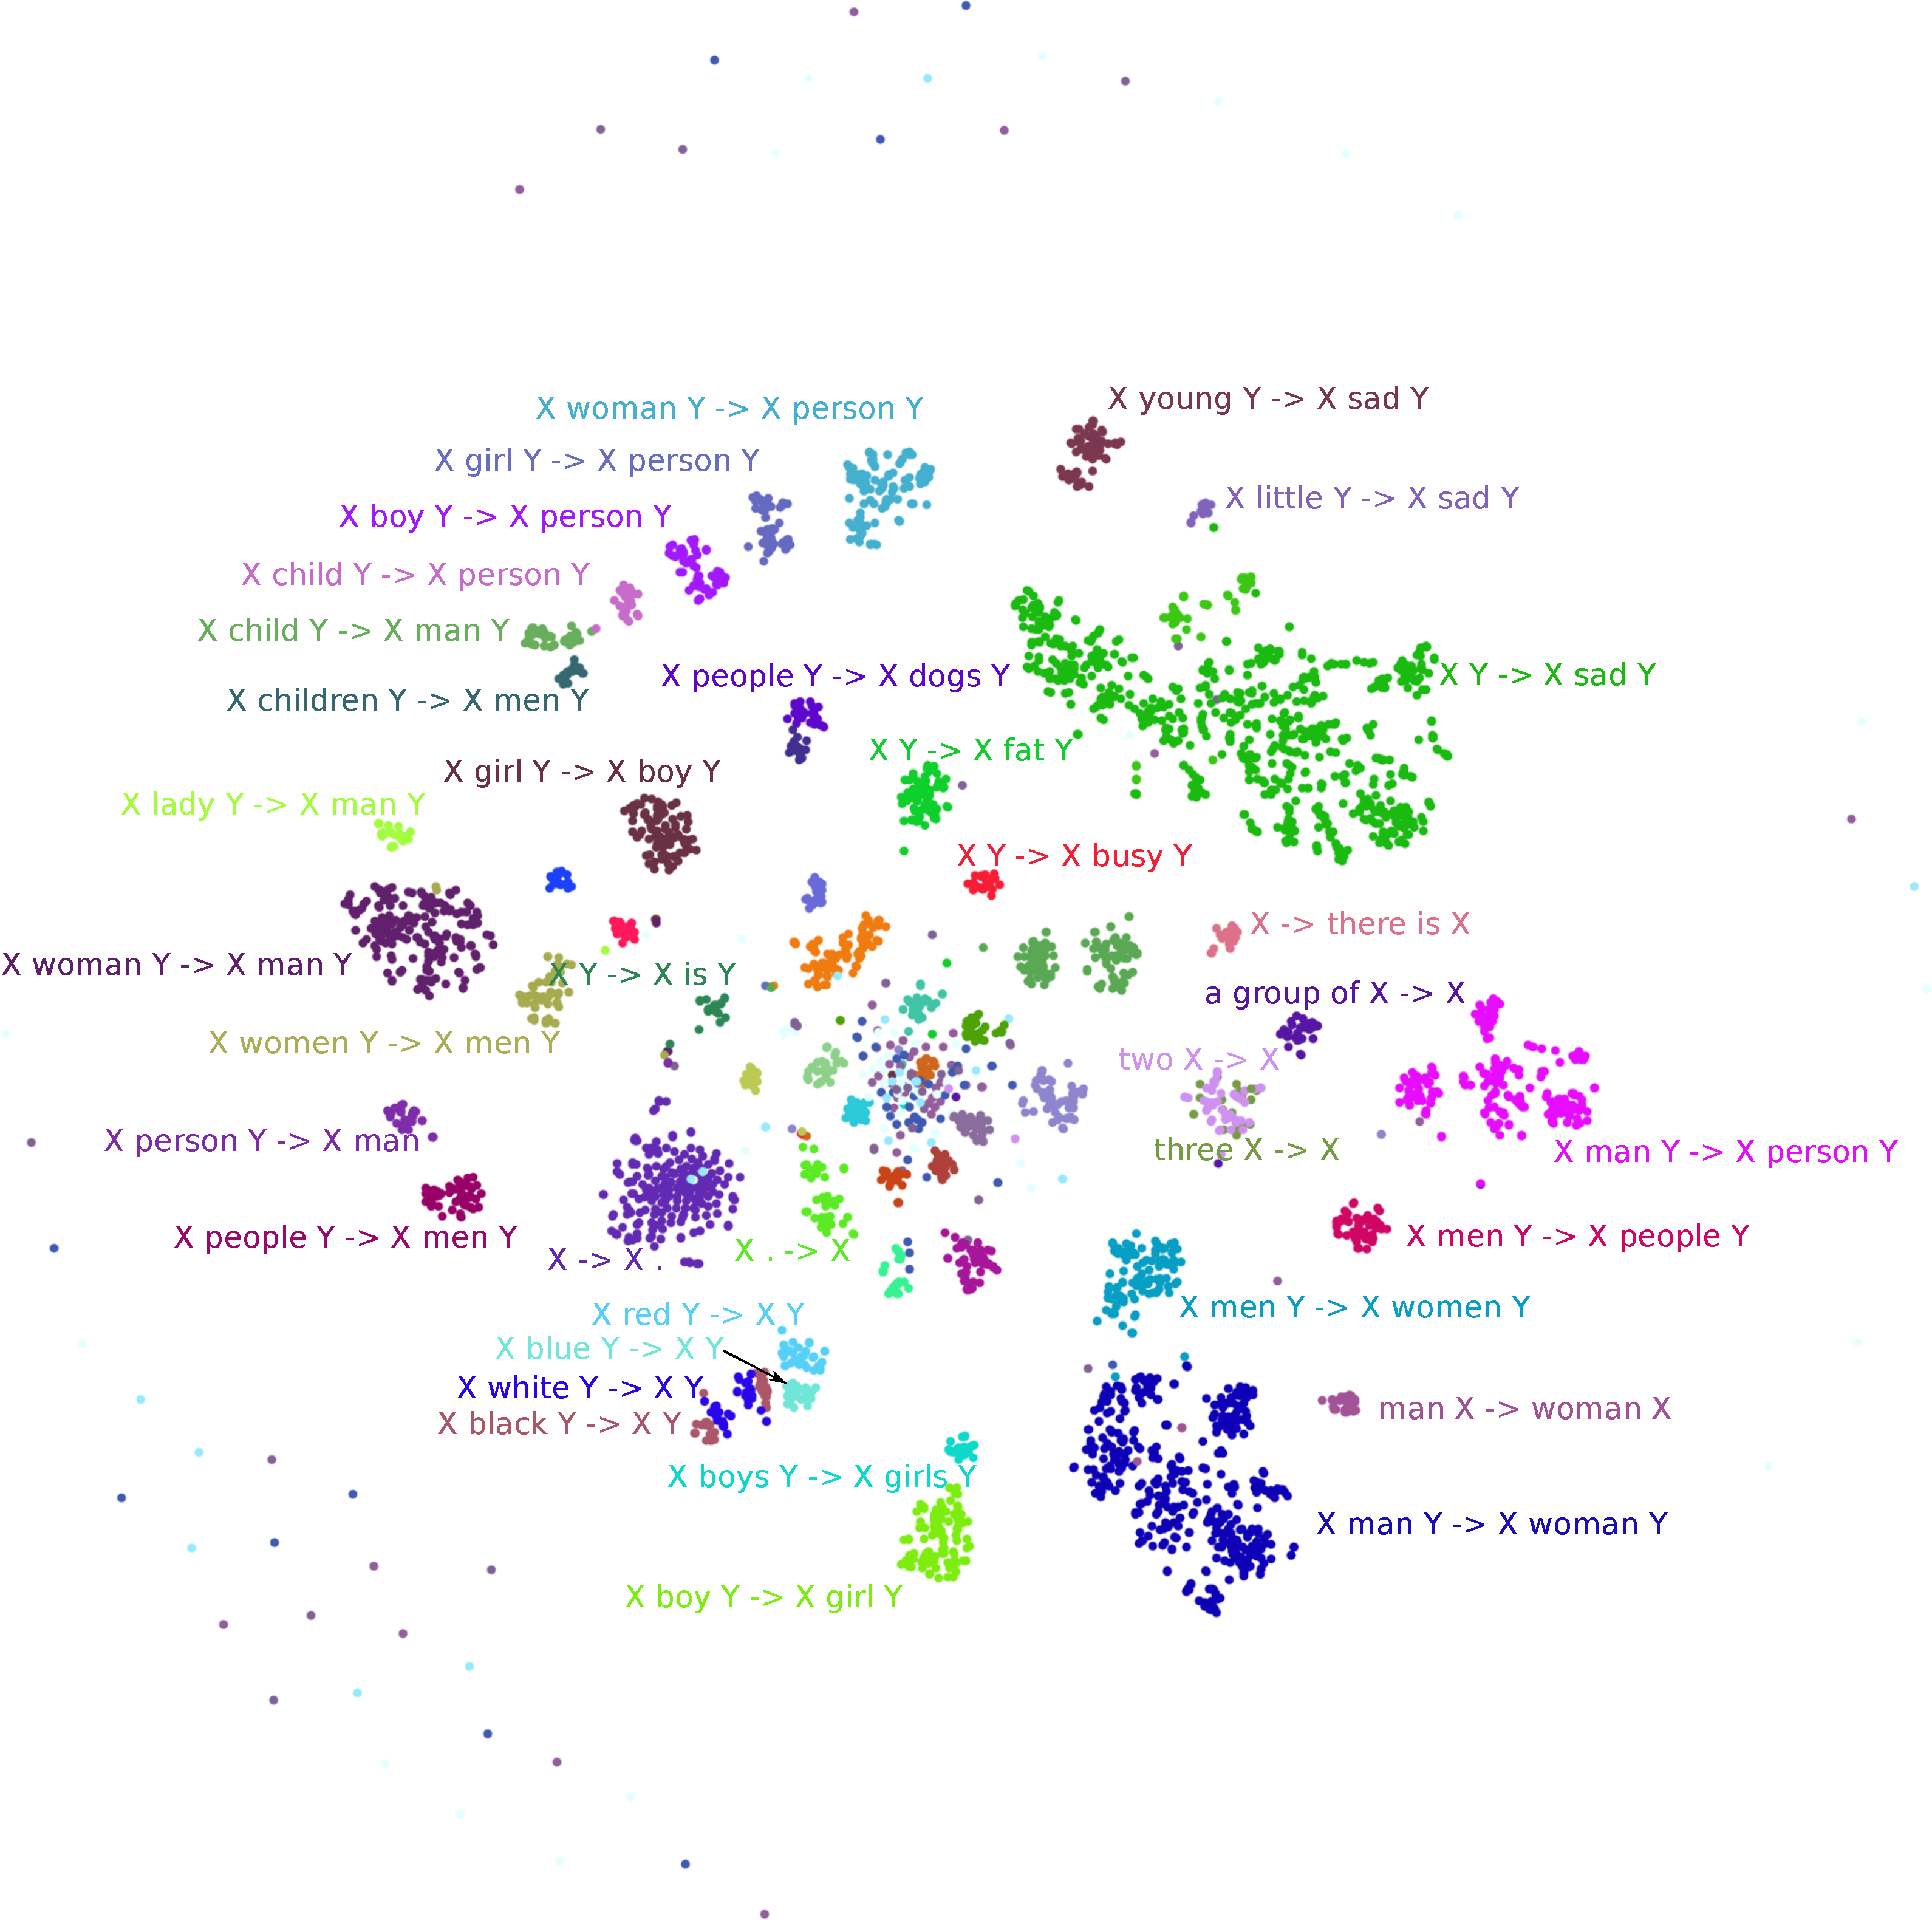
\includegraphics[width=\textwidth]{tsne.pdf}
\caption{The t-SNE visualization of sentence patterns, reprinted from \cite{barancikova-bojar-linear}. Each point in the operation space represents a transformation vector $(v_{hypothesis}-v_{premise})$ derived from \texttt{ELMo} embeddings. Colors denote the specific sentence patterns, with all 60 patterns included. Best viewed in color.}
\label{fig:tsne}
\end{figure}

We visualize the subtraction vectors via t-SNE  \citep{vanDerMaaten2008} in \Cref{fig:tsne} using \elmo as a case study, as this embedding model was not trained using the SNLI dataset. The visualization shows that many patterns form compact clusters without any supervised knowledge of the labels with the exception of a ``chaos cloud'' in the middle and several outliers. There are also several patterns that seem inseparable, e.g. \pattern{two $X$}{$X$} and \pattern{three $X$}{$X$}, or \pattern{$X$ white $Y$}{$X$ $Y$} and \pattern{$X$ black $Y$}{$X$ $Y$},

To better understand the patterns responsible for the noisy center and outliers, we analyze individual patterns using \emph{inertia}, defined here as the mean squared cosine distance between transformation vectors and their centroid in the space of operations. For a pattern with vectors ${v_i}_{i=1}^n$ and centroid $\mu$, we compute:

\[
\frac{1}{n} \sum_{i=1}^{n} (1 - \cos(v_i, \mu))^2.
\]

Lower inertia indicates compact and coherent clusters, whereas higher inertia corresponds to more dispersed or inconsistent transformations.

Our analysis reveals that patterns with the highest inertia are predominantly associated with word-order changes and punctuation insertions or deletions. These patterns correspond to the diffuse central region (“chaos cloud”) and the outliers visible in \Cref{fig:tsne}, rather than forming well-separated clusters. Specifically, these patterns include: 


\begin{center}
    \begin{tabular}{l}
        \pattern{X is Y .}{Y is X} \\
        \pattern{X Y .}{Y X .} \\
        \pattern{X}{X .} \\
        \pattern{X , Y .}{Y X .} \\
        \pattern{X , Y .}{Y , X .} \\
        \pattern{X Y .}{Y , X .} \\
        \pattern{X .}{X}
    \end{tabular}
\end{center}

This suggests that syntactically driven transformations are less consistently represented in the embedding space, leading to higher dispersion, whereas semantically coherent transformations tend to form compact clusters. The failure of subtraction to capture word-order changes (\pattern{X is Y .}{Y is X}) further indicates that \elmo behaves more like a weighted bag-of-words model than true structural encoders in this geometric context.

\bigskip %ML
\noindent %ML 
To investigate whether the space of operations can be interpreted also automatically, i.e., to determine if sentence relations are generalizable, we remove the previously identified noisy patterns selected above and apply fully unsupervised clustering; we do not disclose the expected number of clusters in advance.

To determine the optimal number of clusters, we employ two standard metrics: the Davies-Bouldin's index \citep{Davies} and the Silhouette Coefficient \citep{Rousseeuw:1987}. Both metrics are designed to measure compactness and separation of the clusters, favoring dense and well-separated clusters. Both criteria agree that the best separation is achieved at 9 clusters. Accordingly, we perform k-Means clustering with \(k = 9\).

\begin{figure}[htb!]
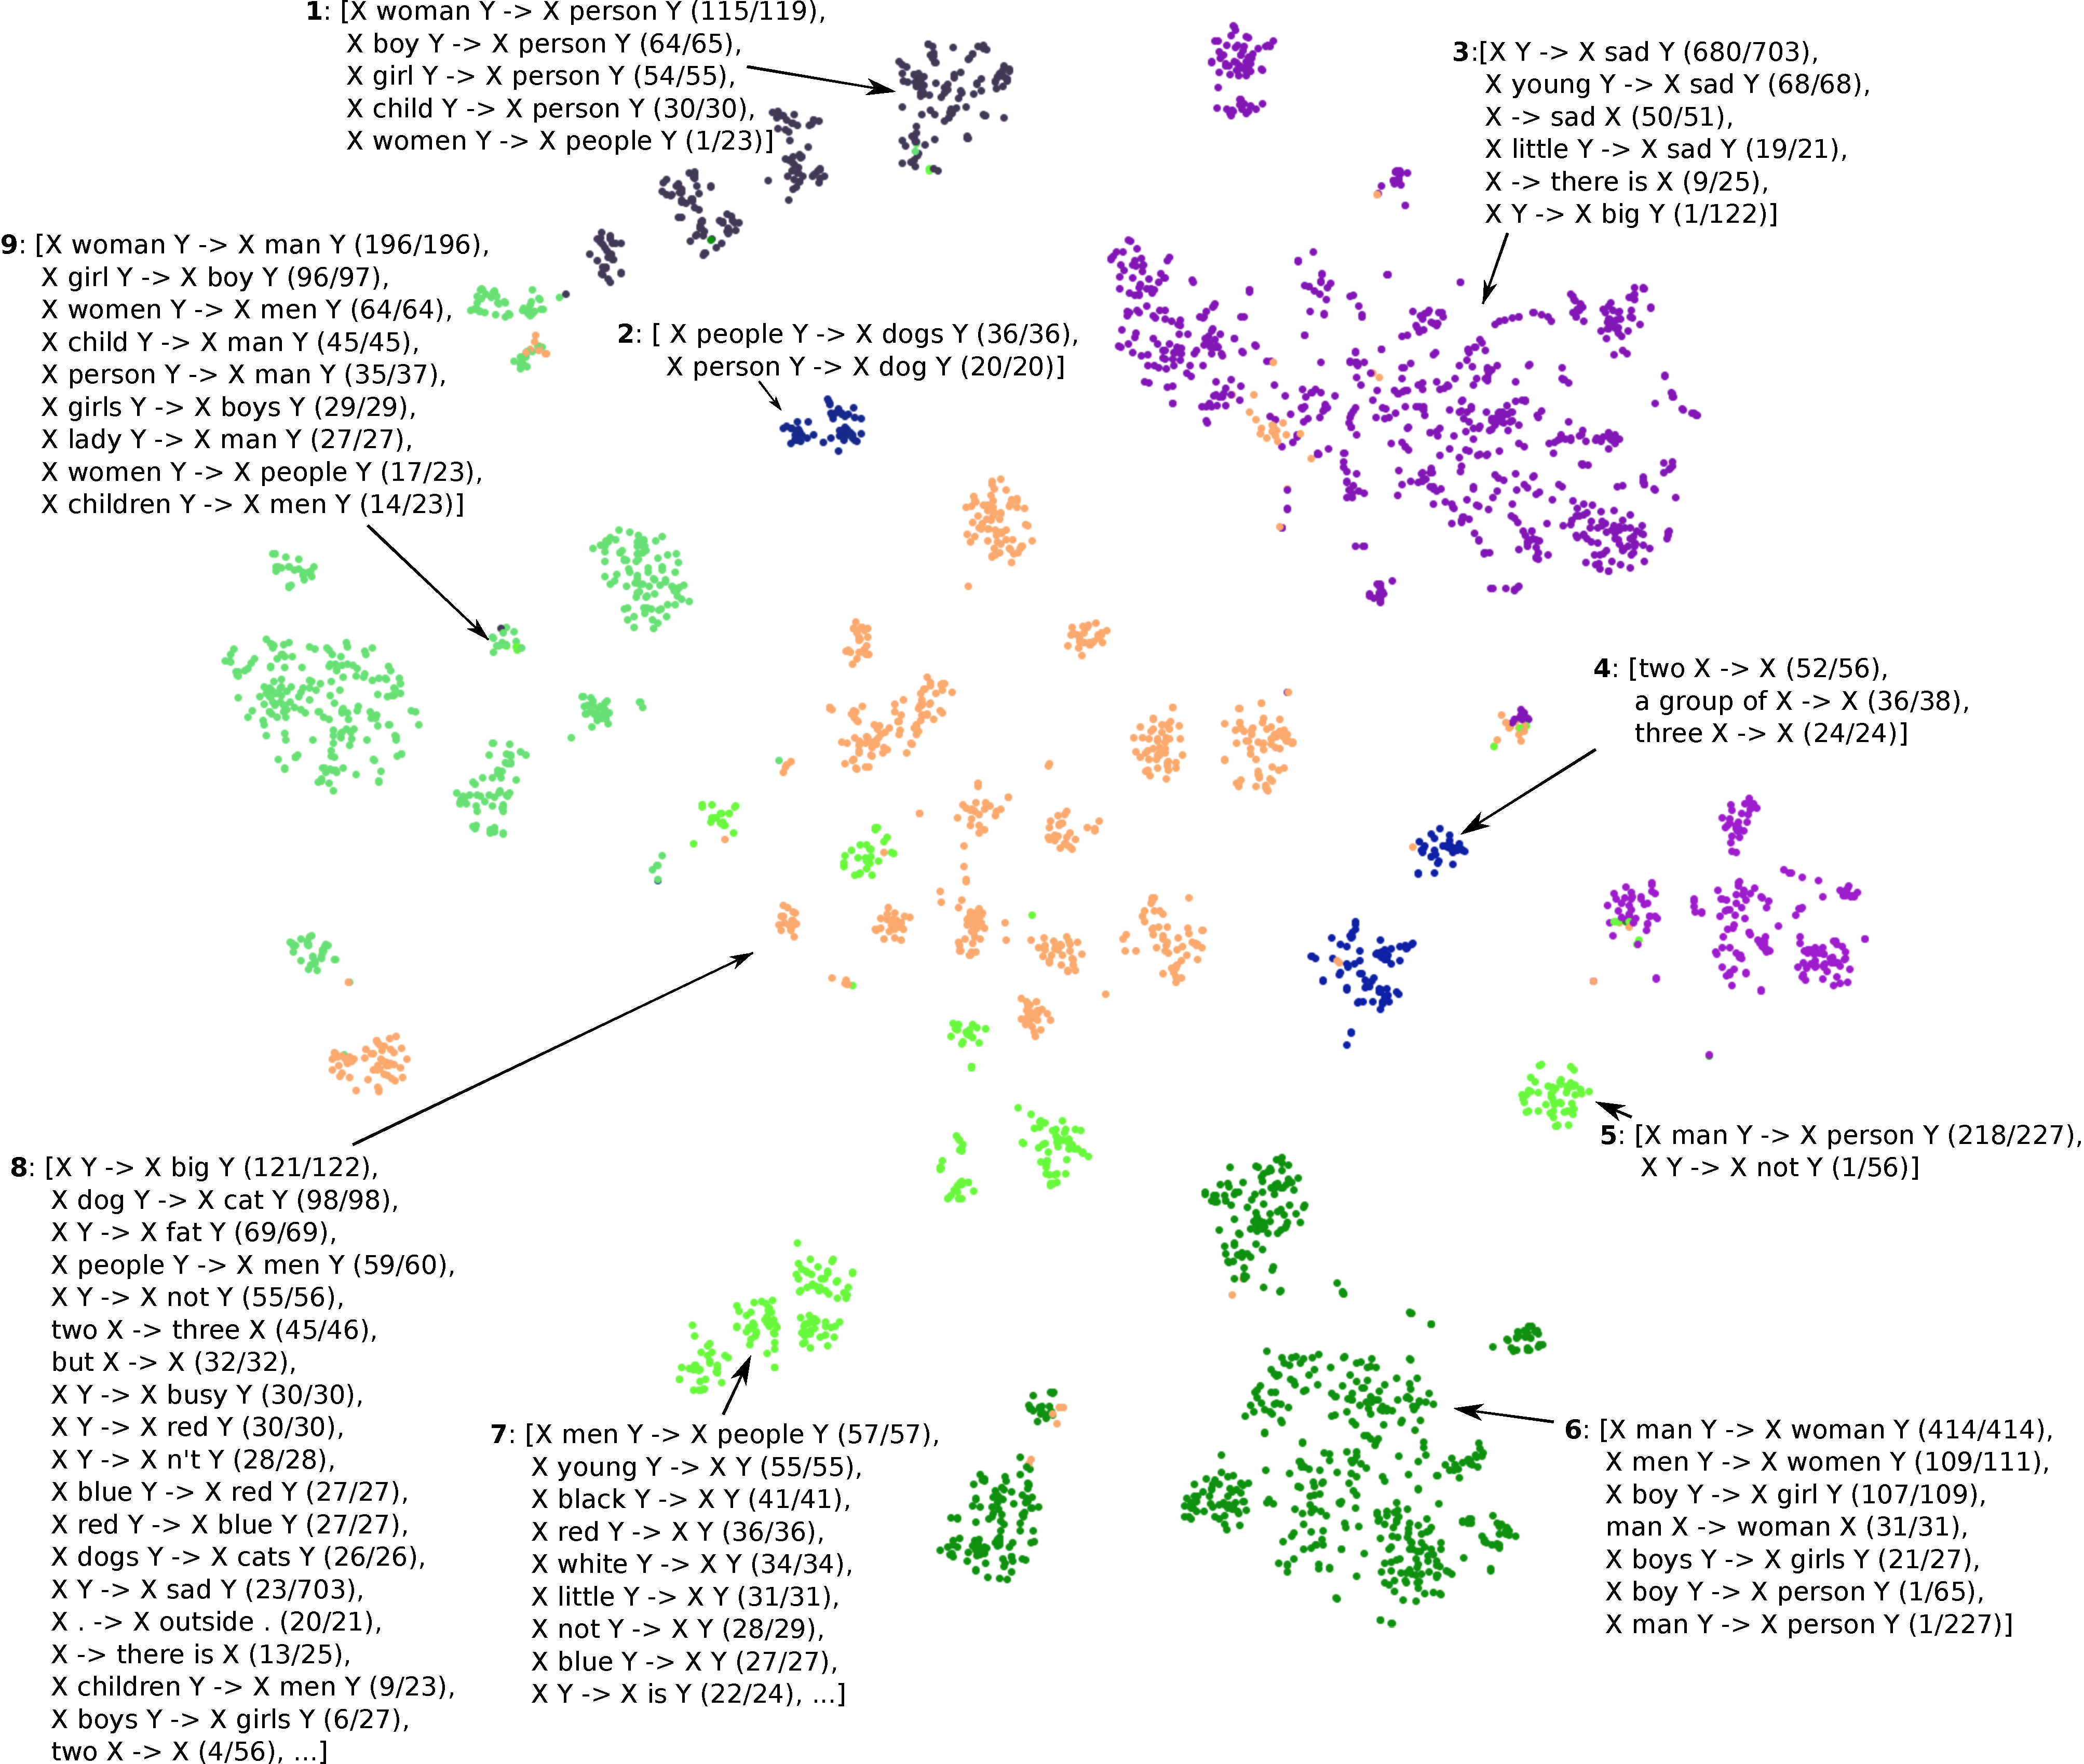
\includegraphics[width=\textwidth]{clustering.pdf}
\caption{The t-SNE visualization of patterns as in \cref{fig:tsne}, with colors representing automatically induced clusters. Each cluster is labelled with the set of patterns extracted from sentence pairs assigned to the cluster. The numbers in parentheses (n/N) indicate the count of sentence pairs belonging to a specific pattern within the cluster (n) relative to the total number of such pairs in the dataset (N). For example, the entry \pattern{two X}{X}(52/56) signifies that of the 56 total sentence pairs differing by the prefix \trans{two}, 52 were grouped into this cluster based on the subtraction of their \texttt{ELMo} embeddings. Reprinted from \cite{barancikova-bojar-linear}.}
\label{fig:clusters}
\end{figure}

The resulting clustering is illustrated in \Cref{fig:clusters}. Manual inspection reveals that many clusters capture coherent and interpretable transformation patterns. For example, Cluster 1 captures 90\% (altogether 264 out of 292) sentence pairs that generalize women, boys, or girls to person. The corresponding generalization for men occurs in Cluster 5 (218 out of 227 pairs) for the singular case, and in Cluster 7 for the plural case. Specifically, Cluster 7 contains all 57 plural pairs of the form \pattern{X men Y} {X people Y}, along with various oppositions. 

Cluster 2 contains all sentence pairs in which a person is replaced with a dog, whereas Cluster 3 is primarily connected with sentence pairs that introduce a negative mood. Cluster 4 unites patterns that represent omitting a numeral or a group of entities. Cluster 6 covers gender oppositions in one direction, and Cluster 9 adds the other direction with some noise related to transformations such as child/man or person/man. Cluster 8 does not exhibit a clearly defined semantic theme and can be interpreted as a residual cluster.

\subsection{Pattern Analysis}
Based on the inertia results of the \elmo model, we continue to evaluate the stability of linguistic patterns across different sentence embedding spaces. By measuring how tightly a model clusters vectors for a specific linguistic transformation (e.g., gender swaps or negation), we can examine the internal consistency of the model and its sensitivity to context.

We exclude the \random baseline from this analysis because its inertia values depend solely on random initialization and therefore do not provide an informative baseline for comparing semantically motivated transformation patterns.

\begin{figure}[tb!]
    \centering
    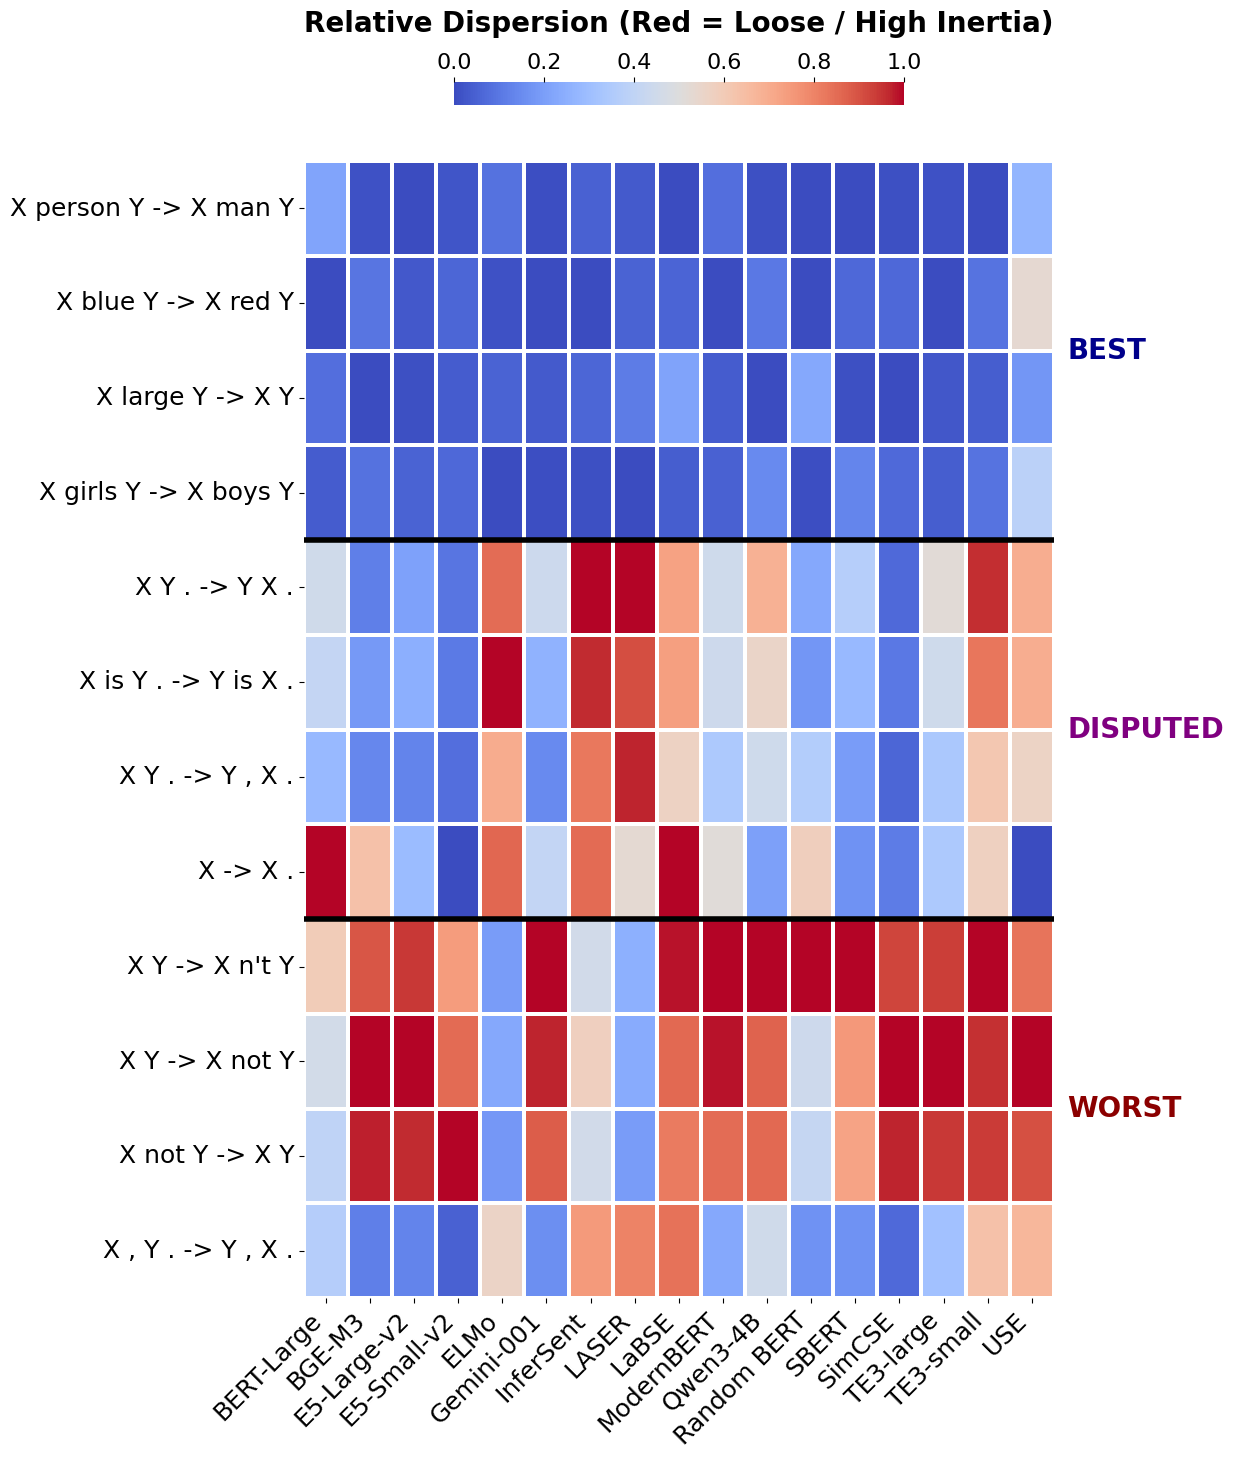
\includegraphics[width=\linewidth]{inertia.png}
    \caption{Example of inertia values for selected patterns across different embedding models. Red color represent patterns with high inertia, which correspond to incoherent, loosely scattered transformation vector in the operation space. Blue indicates compact clusters.}
    \label{fig:inertia}
\end{figure}

In \Cref{fig:inertia}, we visualize a representative subset of patterns selected automatically based on their inertia statistics across models. Specifically, we identify: (i) four patterns with the lowest average inertia (BEST), (ii) four patterns with the highest average inertia (WORST), and (iii) four patterns with the highest variance in inertia across models (DISPUTED). 

\begin{itemize}
\item \textbf{BEST:}
This category comprises patterns with the lowest average inertia (dark blue), indicating a high degree of semantic coherence across models. These transformations induce stable and compact clusters in the embedding space, suggesting that the underlying semantic relations are robustly encoded irrespective of architectural differences.

\item \textbf{DISPUTED:}  
Patterns in this group exhibit substantial variance in inertia across models, revealing pronounced architectural sensitivities. Notably, sentence-order transformations (e.g., \pattern{X is Y .}{Y is X}) dominate this category. Transformer-based models, such as \esmall and \simcse, consistently maintain low inertia, whereas sequential or fixed-encoder architectures (including \elmo, \laser, and \infersent) show markedly higher dispersion. This result is consistent with findings presented by \cite{attention} that demonstrate that self-attention--based architectures are less sensitive to strict sequential order due to their attention-based architecture, allowing more stable representations under syntactic reordering, while LSTM-based encoders are known to be highly sensitive to word order perturbations \citep{conneau2018cram, dasgupta2018}.

\item \textbf{WORST:}  
This category contains patterns with consistently high inertia values (red), which indicates loose or noisy representations. These patterns mainly involve transformations involving negation (e.g., \pattern{X Y }{X not Y}), which systematically disrupt semantic clustering. This finding corresponds to previous evidence that Transformer-based sentence embeddings often place negated sentences close to their affirmative counterparts and perform poorly in negation-sensitive instances \citep{ettinger-2020-bert, hossain-etal-2022-analysis}. In contrast to the \textbf{DISPUTED} category, modern Transformer-based models show the highest inertia, while legacy models such as \elmo, \laser, and \infersent demonstrate relatively greater consistency.

\end{itemize}

%2: $X$ $Y$ -> $X$ sad $Y$ (680/703), $X$ young $Y$ -> $X$ sad $Y$ (68/68), $X$ -> sad $X$ (50/51), $X$ little $Y$ -> $X$ sad $Y$ (19/21), $X$ -> there is $X$ (9/25), $X$ $Y$ -> $X$ big $Y$ (1/122)
%
%5: $X$ woman $Y$ -> $X$ man $Y$ (196/196), $X$ girl $Y$ -> $X$ boy $Y$ (96/97), $X$ women $Y$ -> $X$ men $Y$ (64/64), $X$ child $Y$ -> $X$ man $Y$ (45/45), $X$ person $Y$ -> $X$ man $Y$ (35/37), $X$ girls $Y$ -> $X$ boys $Y$ (29/29), $X$ lady $Y$ -> $X$ man $Y$ (27/27), $X$ women $Y$ -> $X$ people $Y$ (17/23), $X$ children $Y$ -> $X$ men $Y$ (14/23), $X$ woman $Y$ -> $X$ person $Y$ (2/119), $X$ $Y$ -> $X$ is $Y$ (1/24), $X$ girl $Y$ -> $X$ person $Y$ (1/55), $X$ people $Y$ -> $X$ men $Y$ (1/60)
%
%3: $X$ $Y$ -> $X$ big $Y$ (121/122), $X$ dog $Y$ -> $X$ cat $Y$ (98/98), $X$ $Y$ -> $X$ fat $Y$ (69/69), $X$ people $Y$ -> $X$ men $Y$ (59/60), $X$ $Y$ -> $X$ not $Y$ (55/56), two $X$ -> three $X$ (45/46), but $X$ -> $X$ (32/32), $X$ $Y$ -> $X$ busy $Y$ (30/30), $X$ $Y$ -> $X$ red $Y$ (30/30), $X$ $Y$ -> $X$ n't $Y$ (28/28), $X$ blue $Y$ -> $X$ red $Y$ (27/27), $X$ red $Y$ -> $X$ blue $Y$ (27/27), $X$ dogs $Y$ -> $X$ cats $Y$ (26/26), $X$ $Y$ -> $X$ sad $Y$ (23/703), $X$ . -> $X$ outside . (20/21), $X$ -> there is $X$ (13/25), $X$ children $Y$ -> $X$ men $Y$ (9/23), $X$ boys $Y$ -> $X$ girls $Y$ (6/27), two $X$ -> $X$ (4/56), $X$ person $Y$ -> $X$ man $Y$ (2/37), $X$ boy $Y$ -> $X$ girl $Y$ (2/109), $X$ men $Y$ -> $X$ women $Y$ (2/111), $X$ man $Y$ -> $X$ person $Y$ (2/227), $X$ little $Y$ -> $X$ sad $Y$ (2/21), $X$ girl $Y$ -> $X$ boy $Y$ (1/97), $X$ not $Y$ -> $X$ $Y$ (1/29), $X$ $Y$ -> $X$ is $Y$ (1/24), a group of $X$ -> $X$ (1/38), $X$ -> sad $X$ (1/51)
%
%6: $X$ man $Y$ -> $X$ person $Y$ (218/227), $X$ $Y$ -> $X$ not $Y$ (1/56)
%
%4: $X$ man $Y$ -> $X$ woman $Y$ (414/414), $X$ men $Y$ -> $X$ women $Y$ (109/111), $X$ boy $Y$ -> $X$ girl $Y$ (107/109), man $X$ -> woman $X$ (31/31), $X$ boys $Y$ -> $X$ girls $Y$ (21/27), $X$ boy $Y$ -> $X$ person $Y$ (1/65), $X$ man $Y$ -> $X$ person $Y$ (1/227)
%
%1: $X$ men $Y$ -> $X$ people $Y$ (57/57), $X$ young $Y$ -> $X$ $Y$ (55/55), $X$ black $Y$ -> $X$ $Y$ (41/41), $X$ red $Y$ -> $X$ $Y$ (36/36), $X$ white $Y$ -> $X$ $Y$ (34/34), $X$ little $Y$ -> $X$ $Y$ (31/31), $X$ not $Y$ -> $X$ $Y$ (28/29), $X$ blue $Y$ -> $X$ $Y$ (27/27), $X$ $Y$ -> $X$ is $Y$ (22/24), $X$ large $Y$ -> $X$ $Y$ (22/22), $X$ man $Y$ -> $X$ person $Y$ (6/227), $X$ women $Y$ -> $X$ people $Y$ (5/23), $X$ -> there is $X$ (3/25), $X$ woman $Y$ -> $X$ person $Y$ (2/119), two $X$ -> three $X$ (1/46), $X$ . -> $X$ outside . (1/21), a group of $X$ -> $X$ (1/38)
%
%0: $X$ people $Y$ -> $X$ dogs $Y$ (36/36), $X$ person $Y$ -> $X$ dog $Y$ (20/20)
%
%7: $X$ woman $Y$ -> $X$ person $Y$ (115/119), $X$ boy $Y$ -> $X$ person $Y$ (64/65), $X$ girl $Y$ -> $X$ person $Y$ (54/55), $X$ child $Y$ -> $X$ person $Y$ (30/30), $X$ women $Y$ -> $X$ people $Y$ (1/23)
%
%8: two $X$ -> $X$ (52/56), a group of $X$ -> $X$ (36/38), three $X$ -> $X$ (24/24


\subsection{Conclusion}
\label{conclusion}
In this chapter, we investigate the linear geometric properties of sentence embedding spaces across a wide range of architectures, ranging from legacy BiLSTMs to modern decoder-only LLMs. We analyze 4,200 pairs of sentences across 60 distinct transformation patterns. Our primary objective is to determine whether consistent semantic transformations between sentences correspond to simple operations in the embedding space.

Our first results of sixty sentence-edit patterns provide strong empirical support for this hypothesis -- simple linguistic transformations correspond to a consistent directional shift in the embedding spaces. Among the operations tested, vector subtraction significantly outperforms addition, multiplication, and division, producing well-separated clusters that closely align with known sentence modification patterns.

Importantly, this observed linearity is not an artifact of high dimensionality or the Transformer architecture. Although \enrandombert shows geometric regularities, it fails to produce stable semantically aligned transformation vectors. These results suggest that the observed linear structure is learned from semantic supervision. Furthermore, the scale and parameter count of the model do not reliably predict the quality of the linear semantic structure. Smaller contrastively trained models often match or outperform substantially larger proprietary and LLM-based embeddings. This suggests that training objective and representation alignment play a more decisive role than the size of the model.

Unlike the rest of this thesis, the present experiment was conducted exclusively on English data due to the scarcity of similar resources for the Czech language. To address this gap, the following chapter introduces \costra: a novel dataset specifically designed for the thorough testing of Czech sentence embeddings.

\begin{mdframed}[
    linecolor=gray,
    linewidth=2pt,
    roundcorner=5,
    backgroundcolor=gray!5
]
\noindent
In this chapter, we answered the following research questions:

\paragraph{Can semantic and syntactic transformations between sentences be captured through simple arithmetic operations in continuous vector spaces?}
Yes, but only under specific conditions. Our experiments show that vector subtraction is highly effective in isolating linguistic transformations. By subtracting a premise sentence embedding from a hypothesis sentence embedding, a transformation vector that represents the specific change (e.g., gender swap, negation, or generalization) is created.


\paragraph{To what extent do model architecture and scale influence the linearity of the sentence embedding space?}
Surprisingly, model scale (parameter count) is not a reliable predictor of the linearity of the semantic structure. Model architecture and training objective have a stronger impact than model scale. While larger models do not systematically produce more linear or better-structured spaces, models trained with contrastive or sentence-level supervision consistently yield more coherent transformation vectors. The absence of a clear performance gap across architectures further suggests that linearity is a broadly shared property, but its quality depends on how the embedding space is trained.
    
\paragraph{Is the linearity of a model a result of learned semantic understanding or an inherent inductive bias of its architecture?}
It is a combination of both, but semantic training is essential for meaningful structure. Control experiments with randomly initialized models reveal that architectural biases alone can produce weak, consistent geometric patterns (micro-shifts). However, these patterns do not align with true semantic transformations. Only trained models exhibit stable, semantically interpretable directions, indicating that linearity in sentence embeddings is primarily a learned property rather than a byproduct of architecture.

\paragraph{Which linguistic phenomena are most (and least) consistently represented as linear transformations in sentence embeddings?} Lexical substitutions and semantic generalizations (e.g., \pattern{man}{person}) are represented most consistently, forming compact and stable clusters across models. In contrast, transformations involving negation, word order changes, and punctuation exhibit high variability or noise. 

\end{mdframed}


% TODO: JESTLI BUDE CAS: Unfortunately, choosing ELMo as example might not have been the best option -- we compute ELMo embeddings by averaging contextualized word embeddings and majority of the patterns are just removing/adding/changing a single word. Difference between two such sentence embeddings may be a simple difference between the embeddings of the words substituted, depending on the effect of the  contextualization. Thus, the differences in vector space would show rather the word embeddings than the sentence embeddings. 
       
% It should be noted that our search made use of only about 0.5\% of the sentence pairs available in SNLI and MultiNLI. The remaining sentence pairs differ beyond what was extractable automatically using our simple pattern method. A different approach for a fine-grained description of the semantic relation between two sentences would have to be taken for a better exploitation of the available data. \ml{a ma smysl to zkouset s vetsimi daty }

% \ml{V zaveru citujes (Barančíková and Bojar, 2020) - aha, to je TSD. To bude dalsi kousek?}

%Our plans for the long term are to further verify these observations using a more diverse set of vector operations and a larger set of sentence alternations, primarily by extending the set of alternation \emph{types}. We also plan to examine the possibilities of \emph{generating sentence strings} back from the sentence embedding space. If successful, our method could lead to controlled paraphrasing via the continuous space: take an input sentence, embed it, modify the embedding using a vector operation and generate the target sentence in the standard textual from.



